

\bta{2020}



\section{Use of English}

\noindent
\textbf{Directions:}\\
Read the following text. Choose the best word(s) for each numbered blank
and mark A, B, C or D on the ANSWER SHEET. (10 points)



\TiGanSpace


Even if families don't sit down to eat together as frequently as before,
millions of Britons will nonetheless have got a share this weekend of
one of that nation's great traditions: the Sunday roast. \cloze a
cold winter's day, few culinary pleasures can \cloze it. Yet as
we report now, the food police are determined that this \cloze
should be rendered yet another guilty pleasure \cloze to damage
our health.

The Food Standards Authority (FSA) has \cloze a public warning
about the risks of a compound called acrylamide that forms in some foods
cooked \cloze high temperatures. This means that people should
\cloze crisping their roast potatoes, reject thin-crust pizzas
and only \cloze toast their bread. But where is the evidence to
support such alarmist advice? \cloze studies have shown that
acrylamide can cause neurological damage in mice, there is no
\cloze evidence that it causes cancer in humans.

Scientists say the compound is \cloze to cause cancer but have
no hard scientific proof. \cloze the precautionary principle, it
could be argued that it is \cloze to follow the FSA advice.
\cloze , it was rumoured that smoking caused cancer for years
before the evidence was found to prove a \cloze.

Doubtless a piece of boiled beef can always be \cloze up on
Sunday alongside some steamed vegetables, without the Yorkshire pudding
and no wine. But would life be worth living? \cloze , the FSA
says it is not telling people to cut out roast foods \cloze , but
to reduce their lifetime intake. However, their \cloze risks
coming across as being pushy and overprotective. Constant health scares
just \cloze with no one listening.

\newpage
\begin{enumerate}
\item


\fourchoices
{In}
{On}
{Till}
{Towards}

\item


\fourchoices
{match}
{express}
{satisfy}
{influence}

\item


\fourchoices
{patience}
{concern}
{surprise}
{enjoyment}

\item

\fourchoices
{intensified}
{guaranteed}
{compelled}
{privileged}

\item


\fourchoices
{ignored}
{received}
{issued}
{cancelled}


\item


\fourchoices
{under}
{by}
{for}
{at}

\item


\fourchoices
{forget}
{avoid}
{finish}
{regret}

\item


\fourchoices
{easily}
{regularly}
{partially}
{initially}

\item


\fourchoices
{If}
{Since}
{While}
{Unless}



\item

\fourchoices
{conclusive}
{external}
{secondary}
{negative}



\item


\fourchoices
{likely}
{bound}
{insufficient}
{slow}




\item

\fourchoices
{In addition to}
{At the cost of}
{On the basis of}
{In contrast to}



\item

\fourchoices
{interesting}
{fortunate}
{urgent}
{advisable}



\item

\fourchoices
{As usual}
{After all}
{By definition}
{In particular}





\item

\fourchoices
{connection}
{combination}
{resemblance}
{pattern}



\item


\fourchoices
{made}
{used}
{saved}
{served}






\item

\fourchoices
{To be brief}
{For instance}
{To be fair}
{In general}


\item

\fourchoices
{entirely}
{gradually}
{reluctantly}
{carefully}



\item

\fourchoices
{promise}
{competition}
{experience}
{campaign}




\item


\fourchoices
{follow up}
{end up}
{open up}
{pick up}

\end{enumerate}

\vfil

\section{Reading Comprehension}




\noindent
\textbf{Part A}\\
\textbf{Directions:}\\
Read the following four texts. Answer the questions after each text by
choosing A, B, C or
D. Mark your answers on the ANSWER SHEET. (40
points)



\newpage
\subsection{Text 1}


A group of Labour MPs, among them Yvette Cooper, are bringing in the new
year with a call to institute a UK ``town of culture'' award. The
proposal is that it should sit alongside the existing city of culture
title, which was held by Hull in 2017, and has been awarded to Coventry
for 2021. Cooper and her colleagues argue that the success of the crown
for Hull, where it brought in £220m of investment and an avalanche of
arts, ought not to be confined to cities. Britain's towns, it is true,
are not prevented from applying, but they generally lack the resources
to put together a bid to beat their bigger competitors. A town of
culture award could, it is argued, become an annual event, attracting
funding and creating jobs.

Some might see the proposal as a booby prize for the fact that Britain
is no longer able to apply for the much more prestigious title of
European capital of culture, a sought-after award bagged by Glasgow in
1990 and Liverpool in 2008. A cynic might speculate that the UK is on
the verge of disappearing into an endless fever of self-celebration in
its desperation to reinvent itself for the post-Brexit world: after town
of culture, who knows what will follow---village of culture? Suburb of
culture? Hamlet of culture?


It is also wise to recall that such titles are not a cure-all. A badly
run ``year of culture'' washes in and washes out of a place like the
tide, bringing prominence for a spell but leaving no lasting benefits to
the community. The really successful holders of such titles are those
that do a great deal more than fill hotel bedrooms and bring in
high-profile arts events and good press for a year. They transform the
aspirations of the people who live there; they nudge the self-image of
the city into a bolder and more optimistic light. It is hard to get
right, and requires a remarkable degree of vision, as well as
cooperation between city authorities, the private sector, community
groups and cultural organisations. But it can be done: Glasgow's year as
European capital of culture can certainly be seen as one of a complex
series of factors that have turned the city into the powerhouse of art,
music and theatre that it remains today.

A ``town of culture'' could be not just about the arts but about
honouring a town's peculiarities---helping sustain its high street,
supporting local facilities and above all celebrating its people. Jeremy
Wright, the culture secretary, should welcome this positive, hope-filled
proposal, and turn it into action.


\begin{enumerate}[resume]
\item
Cooper and her colleagues argue that a ``town of culture'' award could  \lineread.




\fourchoices
{consolidate the town-city ties in Britain}
{promote cooperation-among Britain's towns}
{increase the economic strength of Britain's towns}
{focus Britain's limited resources on cultural events}



\item
 According to Paragraph 2, the proposal might be regarded by some as \lineread.


\fourchoices
{a sensible compromise}
{a self-deceiving attempt}
{an eye-catching bonus}
{an inaccessible target}



\item
The author suggests that a title holder is successful only if it \lineread.


\fourchoices
{endeavours to maintain its image}
{meets the aspiration of its people}
{brings its local arts to prominence}
{commits to its long-term growth}


\item
 Glasgow is mentioned in Paragraph 3 to present \lineread.


\fourchoices
{a contrasting case}
{a supporting example}
{a background story}
{a related topic}


\item
What is the author's attitude towards the proposal?


\fourchoices
{Skeptical.}
{Objective.}
{Favourable.}
{Critical.}


\end{enumerate}


\newpage
\subsection{Text 2}



Scientific publishing has long been a licence to print money. Scientists
need journals in which to publish their research, so they will supply
the articles without monetary reward. Other scientists perform the
specialised work of peer review also for free, because it is a central
element in the acquisition of status and the production of scientific
knowledge.

With the content of papers secured for free, the publisher needs only
find a market for its journal. Until this century, university libraries
were not very price sensitive. Scientific publishers routinely report
profit margins approaching 40\% on their operations, at a time when the
rest of the publishing industry is in an existential crisis.

The Dutch giant Elsevier, which claims to publish 25\% of the scientific
papers produced in the world, made profits of more than £900m last year,
while UK universities alone spent more than £210 m in 2016 to enable
researchers to access their own publicly funded research; both figures
seem to rise unstoppably despite increasingly desperate efforts to
change them.

The most drastic, an thoroughly illegal, reaction has been the emergence
of Sci-Hub, a kind of global photocopier for scientific papers, set up
in 2012, which now claims to offer access to every paywalled article
published since 2015. The success of Sci-Hub, which relies on
researchers passing on copies they have themselves legally accessed,
shows the legal ecosystem has lost legitimacy among its users and must
be transformed so that it works for all participants.

In Britain the move towards open access publishing has been driven by
funding bodies. In some ways it has been very successful. More than half
of all British scientific research is now published under open access
terms: either freely available from the moment of publication, or
paywalled for a year or more so that the publishers can make a profit
before being placed on general release.

Yet the new system has not yet worked out any cheaper for the
universities. Publishers have responded to the demand that they make
their product free to readers by charging their writers fees to cover
the costs of preparing an article. These range from around £500 to
\$5,000.  A report last year pointed out that the costs both of
subscriptions and of these ``article preparation costs'' had been
steadily rising at a rate above inflation.
In some ways the scientific publishing model resembles the economy of
the social internet: labour is provided free in exchange for the hope of
status, while huge profits are made by a few big firms who run the
market places. In both cases, we need a rebalancing of power.

\begin{enumerate}[resume]
	%\renewcommand{\labelenumi}{\arabic{enumi}.}
	% A(\Alph) a(\alph) I(\Roman) i(\roman) 1(\arabic)
	%设定全局标号series=example	%引用全局变量resume=example
	%[topsep=-0.3em,parsep=-0.3em,itemsep=-0.3em,partopsep=-0.3em]
	%可使用leftmargin调整列表环境左边的空白长度 [leftmargin=0em]
	\item
Scientific publishing is seen as ``a licence to print money'' partly
because \lineread.


\fourchoices
{its funding has enjoyed a steady increase}
{its marketing strategy has been successful}
{its payment for peer review is reduced}
{its content acquisition costs nothing}


\item
According to Paragraphs 2 and 3, scientific publishers Elsevier have \lineread.


\fourchoices
{thrived mainly on university libraries}
{gone through an existential crisis}
{revived the publishing industry}
{financed researchers generously}


\item
How does the author feel about the success of Sci-Hub?


\fourchoices
{Relieved.}
{Puzzled.}
{Concerned.}
{Encouraged.}


\item
 It can be learned from Paragraphs 5 and 6 that open access terms \lineread.


\fourchoices
{allow publishers some room to make money}
{render publishing much easier for scientists}
{reduce the cost of publication substantially}
{free universities from financial burdens}


\item
Which of the following characterizes the scientific publishing
model?


\fourchoices
{Trial subscription is offered.}
{Labour triumphs over status.}
{Costs are well controlled.}
{The few feed on the many.}


\end{enumerate}


\newpage
\subsection{Text 3}


Progressives often support diversity mandates as a path to equality and
a way to level the playing field. But all too often such policies are an
insincere form of virtue-signaling that benefits only the most
privileged and does little to help average people.

A pair of bills sponsored by Massachusetts state Senator Jason Lewis and
House Speaker Pro Tempore Patricia Haddad, to ensure ``gender parity''
on boards and commissions, provide a case in point.


Haddad and Lewis are concerned that more than half the state-government
boards are less than 40 percent female. In order to ensure that elite
women have more such opportunities, they have proposed imposing
government quotas. If the bills become law, state boards and commissions
will be required to set aside 50 percent of board seats for women by 2022.

The bills are similar to a measure recently adopted in Califomia, which
last year became the first state to require gender quotas for private
companies. In signing the measure, California Governor Jerry Brown
admitted that the law, which expressly classifies people on the basis of
sex, is probably unconstitutional.

The US Supreme Court frowns on sex-based classifications unless they are
designed to address an ``important'' policy interest, Because the
California law applies to all boards, even where there is no history of
prior discrimination, courts are likely to rule that the law violates
the constitutional guarantee of ``equal protection''.

But are such government mandates even necessary? Female participation on
corporate boards may not currently mirror the percentage of women in the
general population, but so what?

The number of women on corporate boards has been steadily increasing
without government interference. According to a study by Catalyst,
between 2010 and 2015 the share of women on the boards of global
corporations increased by 54 percent.

Requiring companies to make gender the primary qualification for board
membership will inevitably lead to less experienced private sector
boards. That is exactly what happened when Norway adopted a nationwide
corporate gender quota.

Writing in \emph{The New Republic}, Alice Lee notes that increasing the
number of opportunities for board membership without increasing the pool
of qualified women to serve on such boards has led to a ``golden skirt''
phenomenon, where the same elite women scoop up multiple seats on a
variety of boards.

Next time somebody pushes corporate quotas as a way to promote gender
equity, remember that such policies are largely self-serving measures
that make their sponsors feelgood but do little to help average women.


\begin{enumerate}[resume]
	%\renewcommand{\labelenumi}{\arabic{enumi}.}
	% A(\Alph) a(\alph) I(\Roman) i(\roman) 1(\arabic)
	%设定全局标号series=example	%引用全局变量resume=example
	%[topsep=-0.3em,parsep=-0.3em,itemsep=-0.3em,partopsep=-0.3em]
	%可使用leftmargin调整列表环境左边的空白长度 [leftmargin=0em]
	\item
The author believes that the bills sponsored by Lewis and Haddad will \lineread.


\fourchoices
{help little to reduce gender bias}
{pose a threat to the state government}
{raise women's position in politics}
{greatly broaden career options}


\item
 Which of the following is true of the Califormia measure?


\fourchoices
{It has irritated private business owners.}
{It is welcomed by the Supreme Court.}
{It may go against the Constitution.}
{It will settle the prior controversies.}


\item
 The author mentions the study by Catalyst to illustrate \lineread.


\fourchoices
{the harm from arbitrary board decision}
{the importance of constitutional guarantees}
{the pressure on women in global corporations}
{the needlessness of government interventions}


\item
Norway's adoption of a nationwide corporate gender quota has led to \lineread.


\fourchoices
{the underestimation of elite women's role}
{the objection to female participation on boards}
{the entry of unqualified candidates into the board}
{the growing tension between labor and management}



\item
 Which of the following can be inferred from the text?


\fourchoices
{Women's need in employment should be considered.}
{Feasibility should be a prime concern in policymaking.}
{Everyone should try hard to promote social justice.}
{Major social issues should be the focus of legislation.}

\end{enumerate}



\newpage
\subsection{Text 4}


Last Thursday, the French Senate passed a digital services tax, which
would impose an entirely new tax on large multinationals that provide
digital services to consumers or users in France. Digital services
include everything from providing a platform for selling goods and
services online to targeting advertising based on user data, and the tax
applies to gross revenue from such services. Many French politicians and
media outlets have referred to this as a `` GAFA tax,'' meaning that it
is designed to apply primarily to companies such as Google, Apple,
Facebook and Amazon---in other words, multinational tech companies based
in the United States.

The digital services tax now awaits the signature of President Emmanuel
Macron, who has expressed support for the measure, and it could go into
effect within the next few weeks. But it has already sparked significant
controversy, with the United States trade representative opening an
investigation into whether the tax discriminates against American
companies, which in tum could lead to trade sanctions against France.

The French tax is not just a unilateral move by one country in need of
revenue.
Instead, the digital services tax is part of a much larger trend, with
countries over the past few years proposing or putting in place an
alphabet soup of new international tax provisions. They have included
Britain's DPT. (diverted profits tax), Australia's MAAL (multinational
anti-avoidance law), and India's SEP (significant economic presence)
test, to name but a few. At the same time, the European Union, Spain,
Britain and several other countries have all seriously contemplated
digital services taxes.

These unilateral developments differ in their specifics, but they are
all designed to tax multinationals on income and revenue that countries
believe they should have a right to tax, even if international tax rules
do not grant them that right. In other words, they all share a view that
the international tax system has failed to keep up with the current
economy.

In response to these many unilateral measures, the Organization for
Economic Cooperation and Development (OECD) is currently working with
131 countries to reach a consensus by the end of 2020 on an
international solution. Both France and the United States are involved
in the organization's work, but France's digital services tax and the
American response raise questions about what the future holds for the
international tax system.

France's planned tax is a clear warning: Unless a broad consensus can be
reached on reforming the international tax system, other nations are
likely to follow suit, and American companies will face a cascade of
different taxes from dozens of nations that will prove burdensome and
costly.

\begin{enumerate}[resume]
	%\renewcommand{\labelenumi}{\arabic{enumi}.}
	% A(\Alph) a(\alph) I(\Roman) i(\roman) 1(\arabic)
	%设定全局标号series=example	%引用全局变量resume=example
	%[topsep=-0.3em,parsep=-0.3em,itemsep=-0.3em,partopsep=-0.3em]
	%可使用leftmargin调整列表环境左边的空白长度 [leftmargin=0em]
	\item
The French Senate has passed a bill to \lineread.


\fourchoices
{regulate digital services platforms}
{protect French companies'' interests}
{impose a levy on tech multinationals}
{curb the influence of advertising}


\item
It can be learned from Paragraph 2 that the digital services tax \lineread.


\fourchoices
{may trigger countermeasures against France}
{is apt to arouse criticism at home and abroad}
{aims to ease international trade tensions}
{will prompt the tech giants to quit France}


\item
The countries adopting the unilateral measures share the opinion
that \lineread.


\fourchoices
{redistribution of tech giants' revenue must be ensured}
{the current international tax system needs upgrading}
{tech multinationals' monopoly should be prevented}
{all countries ought to enjoy equal taxing rights}


\item
It can be learned from Paragraph 5 that the OECD's current work \lineread.


\fourchoices
{is being resisted by US companies}
{needs to be readjusted immediately}
{is faced with uncertain prospects}
{needs to in involve more countries}


\item
Which of the following might be the best title for this text?


\fourchoices
{France Is Confronted with Trade Sanctions}
{France leads the charge on Digital Tax}
{France Says ``NO'' to Tech Multinationals}
{France Demands a Role in the Digital Economy}


\end{enumerate}

\newpage
\noindent
\textbf{Part B}\\
\textbf{Directions:}\\
Read the following text and answer the questions by choosing the most
suitable subheading from the list A-G for each of the numbered
paragraphs (41-45). There are two extra subheadings. Mark your answers
on the ANSWER SHEET. (10 points)


\begin{listmatch}
\item 
Eye fixations are brief


\item 
Too much eye contact is instinctively felt to be rude


\item 
Eye contact can be a friendly social signal


\item 
Personality can affect how a person reacts to eye contact


\item 
Biological factors behind eye contact are being investigated


\item 
Most people are not comfortable holding eye contact with
strangers


\item 
Eye contact can also be aggressive.
\end{listmatch}




In a social situation, eye contact with another person can show that you
are paying attention in a friendly way. But it can also be antagonistic
such as when a political candidate turns toward their competitor during
a debate and makes eye contact that signals hostility. Here's what hard
science reveals about eye contact:

\linefill.

We know that a typical infant will instinctively gaze into its mother's
eyes, and she will look back. This mutual gaze is a major part of the
attachment between mother and child. In adulthood, looking someone else
in a pleasant way can be a complimentary sign of paying attention. It
can catch someone's attention in a crowded room, ``Eye contact and
smile'' can signal availability and confidence, a common-sense notion
supported in studies by psychologist Monica Moore.

\linefill.

Neuroscientist Bonnie Auyeung found that the hormone oxytocin increased
the amount of eye contact from men toward the interviewer during a brief
interview when the direction of their gaze was recorded. This was also
found in high-functioning men with some autistic spectrum symptoms, who
may tend to avoid eye contact. Specific brain regions that respond
during direct gaze are being explored by other researches, using
advanced methods of brain scanning.


\linefill.

With the use of eye-tracking technology, Julia Minson of the Harvard
Kennedy School of Government concluded that eye contact can signal very
different kinds of messages, depending on the situation. While eye
contact may be a sign of connection or trust in friendly situations,
it's more likely to be associated with dominance or intimidation in
adversarial situations. ``Whether you're a politician or a parent, it
might be helpful to keep in mind that trying to maintain eye contact may
backfire if you're trying to convince someone who has a different set of
beliefs than you,''said Minson.


\linefill.

When we look at a face or a picture, our eyes pause on one spot at a
time, often on the eyes or mouth. These pauses typically occur at about
three per second, and the eyes then jump to another spot, until several
important points in the image are registered like a series of snapshots.
How the whole image is then assembled and perceived is still a mystery
although it is the subject of current research.


\linefill.

In people who score high in a test of neuroticism, a personality
dimension associated with self-consciousness and anxiety, eye contact
triggered more activity associated with avoidance, according to the
Finnish researcher Jari Hietanen and colleagues ``Our findings indicate
that people do not only feel different when they are the centre of
attention but that their brain reactions also differ.'' A more direct
finding is that people who scored highly for negative emotions like
anxiety looked at others for shorter periods of time and reported more
comfortable feelings when others did not look directly at them.


\newpage
\noindent
\textbf{Part C}\\
\textbf{Directions:}\\
Read the following text carefully and then translate the underlined
segments into Chinese.   Written your answer on the
ANSWER SHEET. (10 points)


\TiGanSpace

Following the explosion of creativity in Florence during the 14th
century known as the Renaissance, the modern world saw a departure from
what it had once known. It turned from God and the authority of the
Roman Catholic Church and instead favoured a more humanistic approach to
being. Renaissance ideas had spread throughout Europe well into the 17th
century, with the arts and sciences flourishing extraordinarily among
those with a more logical disposition. \transnum \uline{with the Church's
teachings and ways of thinking eclipsed by the Renaissance, the gap
between the Medieval and modern periods had been bridged leading to new
and unexplored intellectual territories.}

During the Renaissance, the great minds of Nicolaus Copernicus, Johannes
Kepler and Galileo Galilei demonstrated the power of scientific study
and discovery. \transnum \uline{Before each of their revelations many
thinkers at the time had sustained more ancient ways of thinking,
including the geocentric view that the Earth was at the centre of our
universe.} Copernicus theorized in 1543 that all of the planets that we
knew of revolved not around the Earth, but the Sun, a system that was
later upheld by Galileo at his own expense. Offering up such a theory
during a time of high tension between scientific and religious minds was
branded as heresy and any such heretics that continued to spread these
lies were to be punished by imprisonment or even death.


\transnum \uline{Despite attempts by the Church to suppress. this new
generation of logicians and rationalists, more explanations for how the
universe functioned were being made at a rate that the people could no
longer ignore}. It was with these great revelations that a new kind of
philosophy founded in reason was born.

The Church's long-standing dogma was losing the great battle for truth
to rationalists and scientists. This very fact embodied the new ways of
thinking that swept through Europe during most of 17th century. (49)
\uline{As many took on the duty of trying to integrate reasoning and
scientific philosophies into the world, the Renaissance was over and it
was time for a new era - the Age of Reason.}

The 17th and 18th centuries were times of radical change and curiosity,
Scientific method, reductionism and the questioning of Church ideals was
to be encouraged, as were ideas of liberty, tolerance and progress. (50)
\uline{Such actions to seek knowledge and to understand what
information we already knew were captured by the Latin phrase `sapere
aude' or `dare to know',} after Immanuel Kant used it in his essay
\emph{An Answer to the Question}: \emph{What is Enlightenment?}. It was
the purpose and responsibility of great minds to go forth and seek out
the truth, which they believed to be founded in knowledge.


\newpage
\section{Writing}



\noindent
\textbf{Part A}\\
\textbf{51. Directions:}


The Students Union of your university has assigned you to inform the
international students about an upcoming singing contest. Write a notice
in about 100 words.

Write your answer on the ANSWER SHEET.

\textbf{Do not} use your own name in the notice. (10 points)


\vspace{2em}

\noindent
\textbf{Part B}\\
\textbf{52. Directions:}



Write an essay of 160-200 words based on the picture below. In your
essay, you should

\begin{listwrite}
	\item 
	 describe the picture briefly,
	
	\item 
	 interpret the implied meaning, and
	
	\item 
	 give your comments.
\end{listwrite}


You should write neatly on the ANSWER SHEET. (20 points)


\begin{figure}[h!]
	\centering
	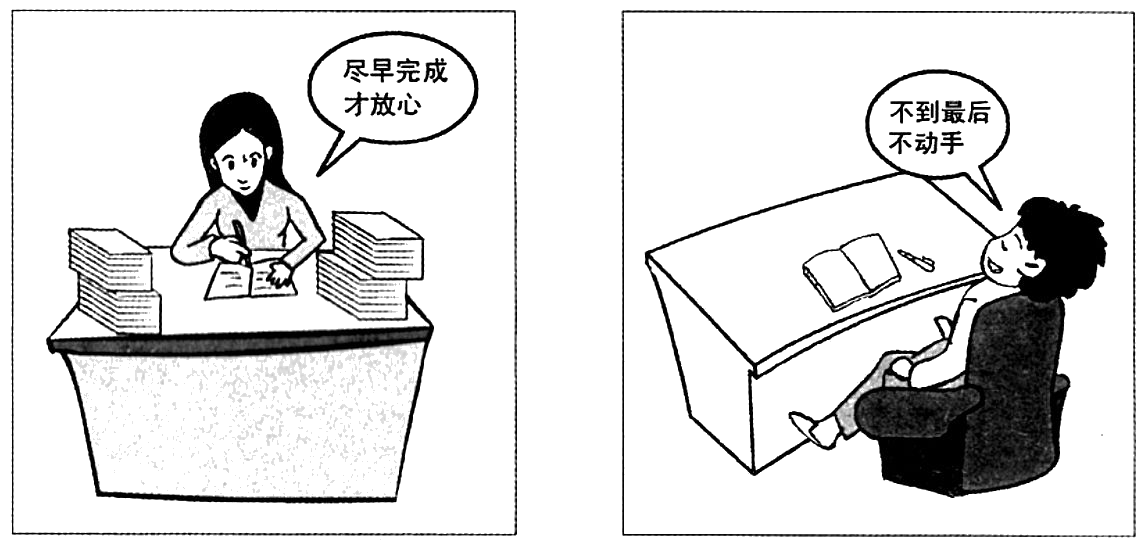
\includegraphics[width=0.76\linewidth]{picture/2020.png}
	\caption*{习惯}
\end{figure}




